\chapter{Adding Figures To Your Document}

\section{My First Figure}

Adding figures is easy in LaTeX. You just create a figure environment which is much the same as the table environment. For example:

\begin{verbatim}
\begin{figure}[!th]
	\centering
	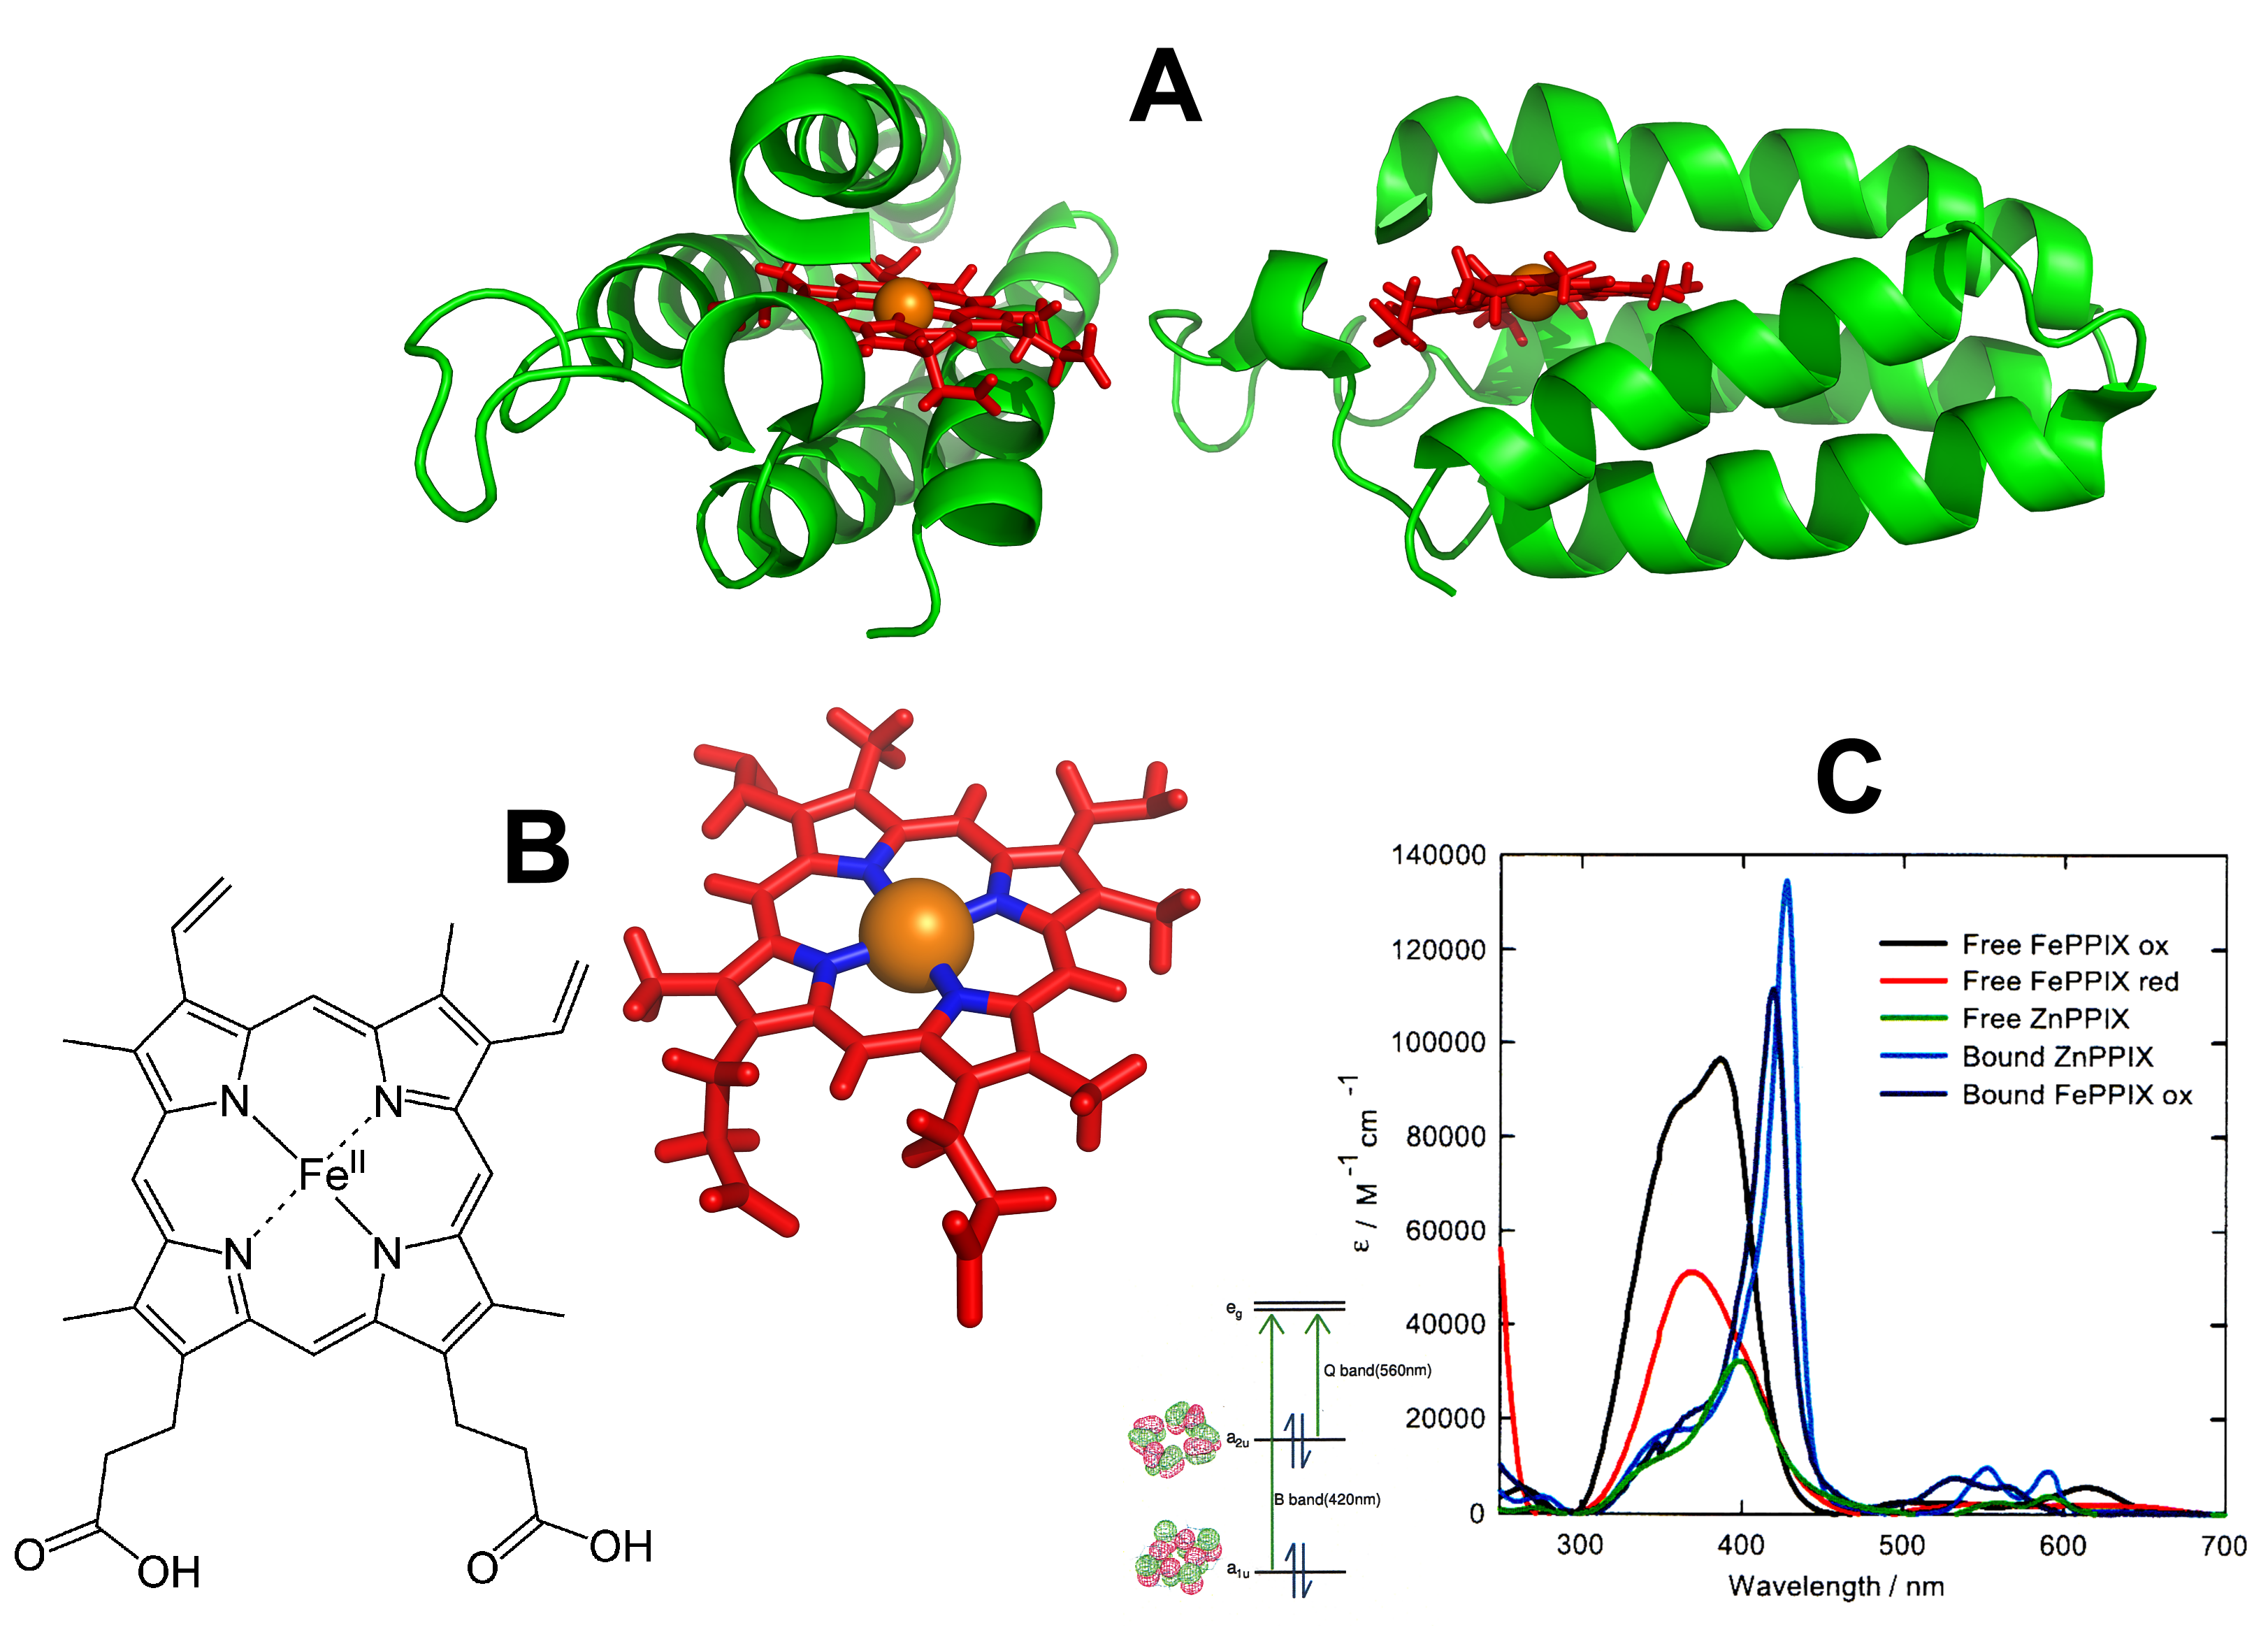
\includegraphics[width=137.4mm]{Images/haemStructure.png}
	\caption[Haem Structure]{A fancy image from Chris' Thesis.}
	\label{fig:haemStructure}
\end{figure}
\end{verbatim}

\vspace{2ex}

\begin{figure}[!th]
	\centering
	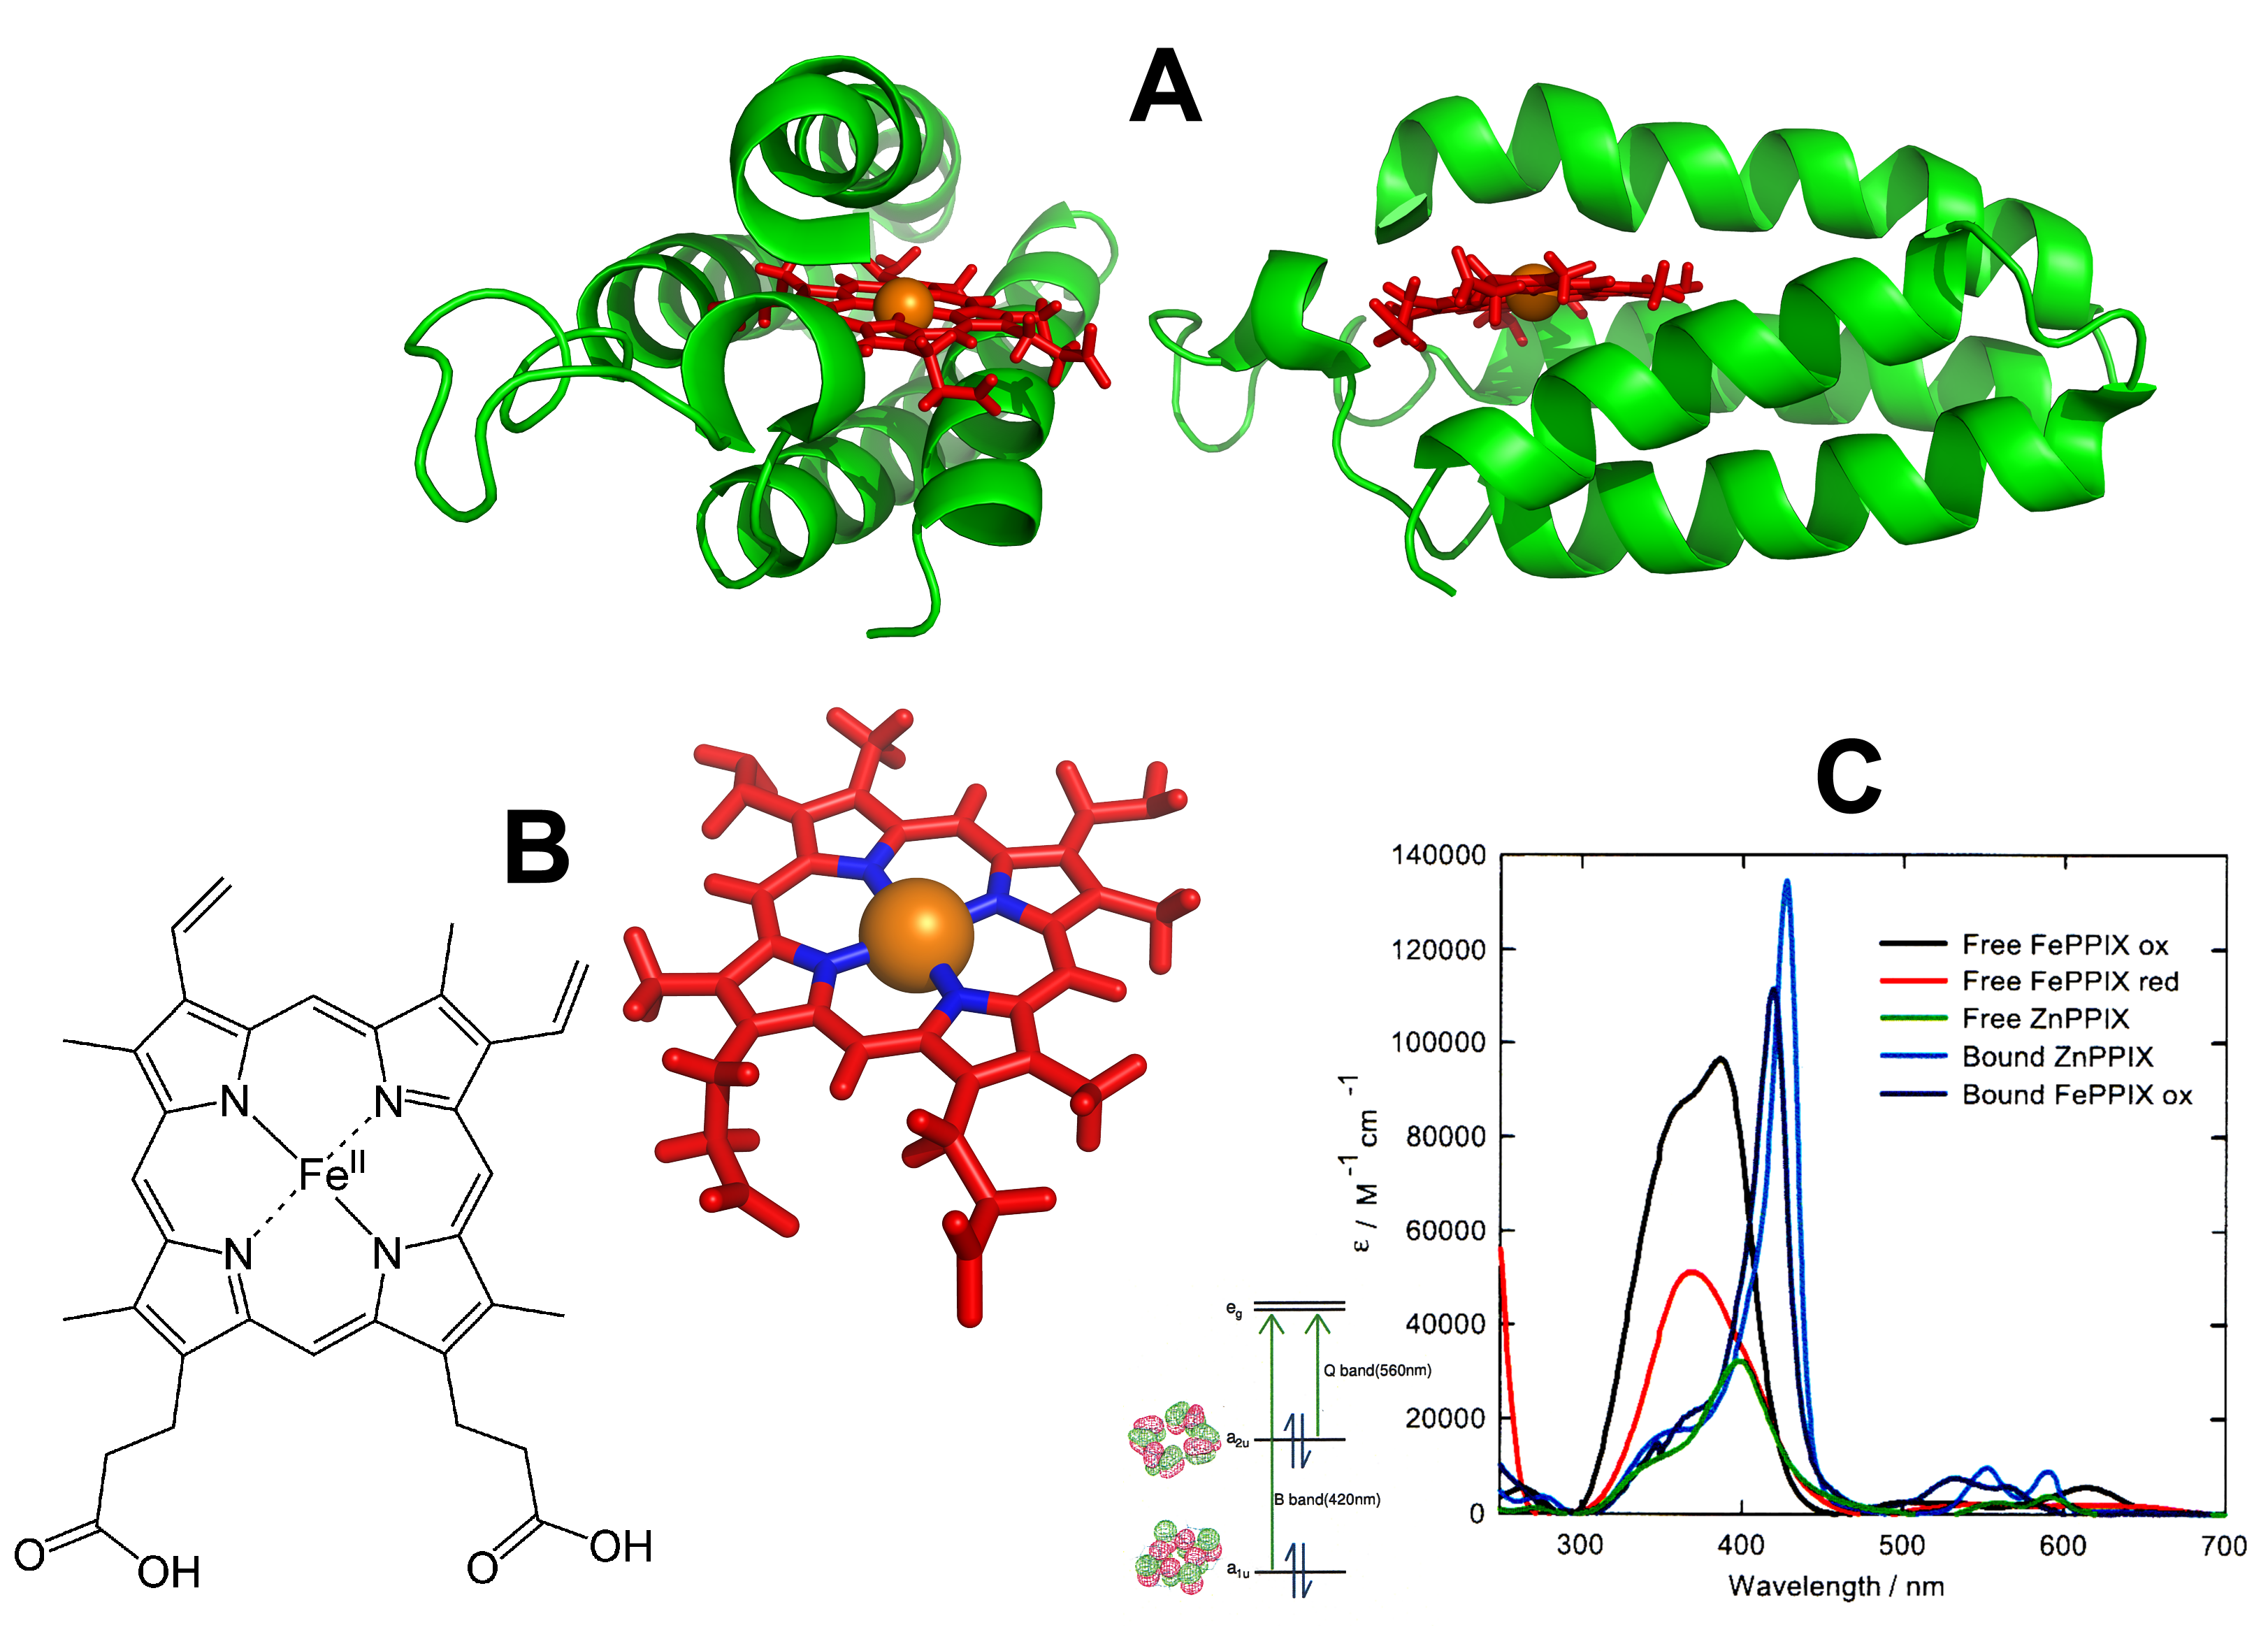
\includegraphics[width=137.4mm]{Images/haemStructure.png}
	\caption[Haem Structure]{A fancy image from Chris' Thesis.}
	\label{fig:haemStructure}
\end{figure}

In this example the command {\textbackslash}includegraphics tells LaTeX to look in the directory `Images' and incorporate the file called `haemStructure.png' into the final document while setting the width to 137.4mm.  This command can be used to resize a graphical file using the height or width parameter as shown. You must specify the units which can be pt, ex, em, mm, cm and so on. LaTeX recognises a very wide variety of standard units and graphics formats. The command is part of the graphicx package and so in the preamble you must include the command {\textbackslash}usepackage\{graphicx\}.

Many packages have been written to provide new commands. For example the `subfigure' package enables you to place separate images or files in the same figure side by side while giving them their own label. However, in this document we only concentrate on the very basics.

\section{Floating Environments}

Both tables and figures are examples of a `floating environments' which means LaTeX decides where to put them. 

The mysterious [!tbh] letters appearing everywhere give guidance to LaTeX about roughly where the figure or table is  allowed to be, but in general they can move a long way from where you position them within your text file.  The letters in the square bracket can be t, h or b which stand for top, here or bottom.  If you don't specify any letters LaTeX defaults to [t].

LaTeX will always preserve the order in which figures appear.  If it cannot find a type setting solution, then it may move the float to it's own page, and combine it with other figures. If it still can't fit that in for some reason then it moves the float to the end of the document.  This has the effect of pushing all the remaining floating environments to the end of the document also.

The exclamation mark instructs LaTeX to ``try harder'' at putting the float where you told it to. Often you must play around to ensure the float positioning is acceptable, but usually this can be achieved by stretching or shrinking the image slightly using the size parameter, re-ordering text, judicial applications of the {\textbackslash}pagebreak command or by shouting loudly and slapping the computer monitor about.